
\section{Results}

\subsection{Simulation Results}

We begin by illustrating the performance of the \textit{CorShrink} method on simulated data. We tested our method on randomly generated covariance matrices of varying dimensions and also on structured matrices- for e.g., block diagonal matrices. We first demonstrate results from applying our models on a block diagonal matrix of dimension $100$. We assumed the block diagonal matrix to be of the form 

\begin{equation}
\begin{pmatrix}
0.2 \mathbf{I} + 0.8 \mathbf{e} \mathbf{e}^{T}   &             0  \\
  0                             &     0.7 \mathbf{I} + 0.3 \mathbf{e}  \mathbf{e}^{T} 
\end{pmatrix}
\end{equation}
 
where $\mathbf{I}$ is the identity matrix and $\mathbf{e}$ is the vector of all $1$'s. We considered four choices of number of samples drawn, $n = 5, 10, 50, 200$ spanning all three scenarios -  $n << p$, $n <p$ and $ n > p$.  We then estimated the correlation matrix using three versions of \textit{CorShrink}, GLASSO at four different regularization parameter values ranging from low to high shrinkage and the Sch\"{a}fer-Strimmer method (see Friedman et al (2008) \cite{Friedman2008}, Witten et al (2010) \cite{Witten2010} and Sch\"{a}fer-Strimmer (2005) \cite{Schafer2005}). 

\begin{figure*}[ht]
\raggedleft
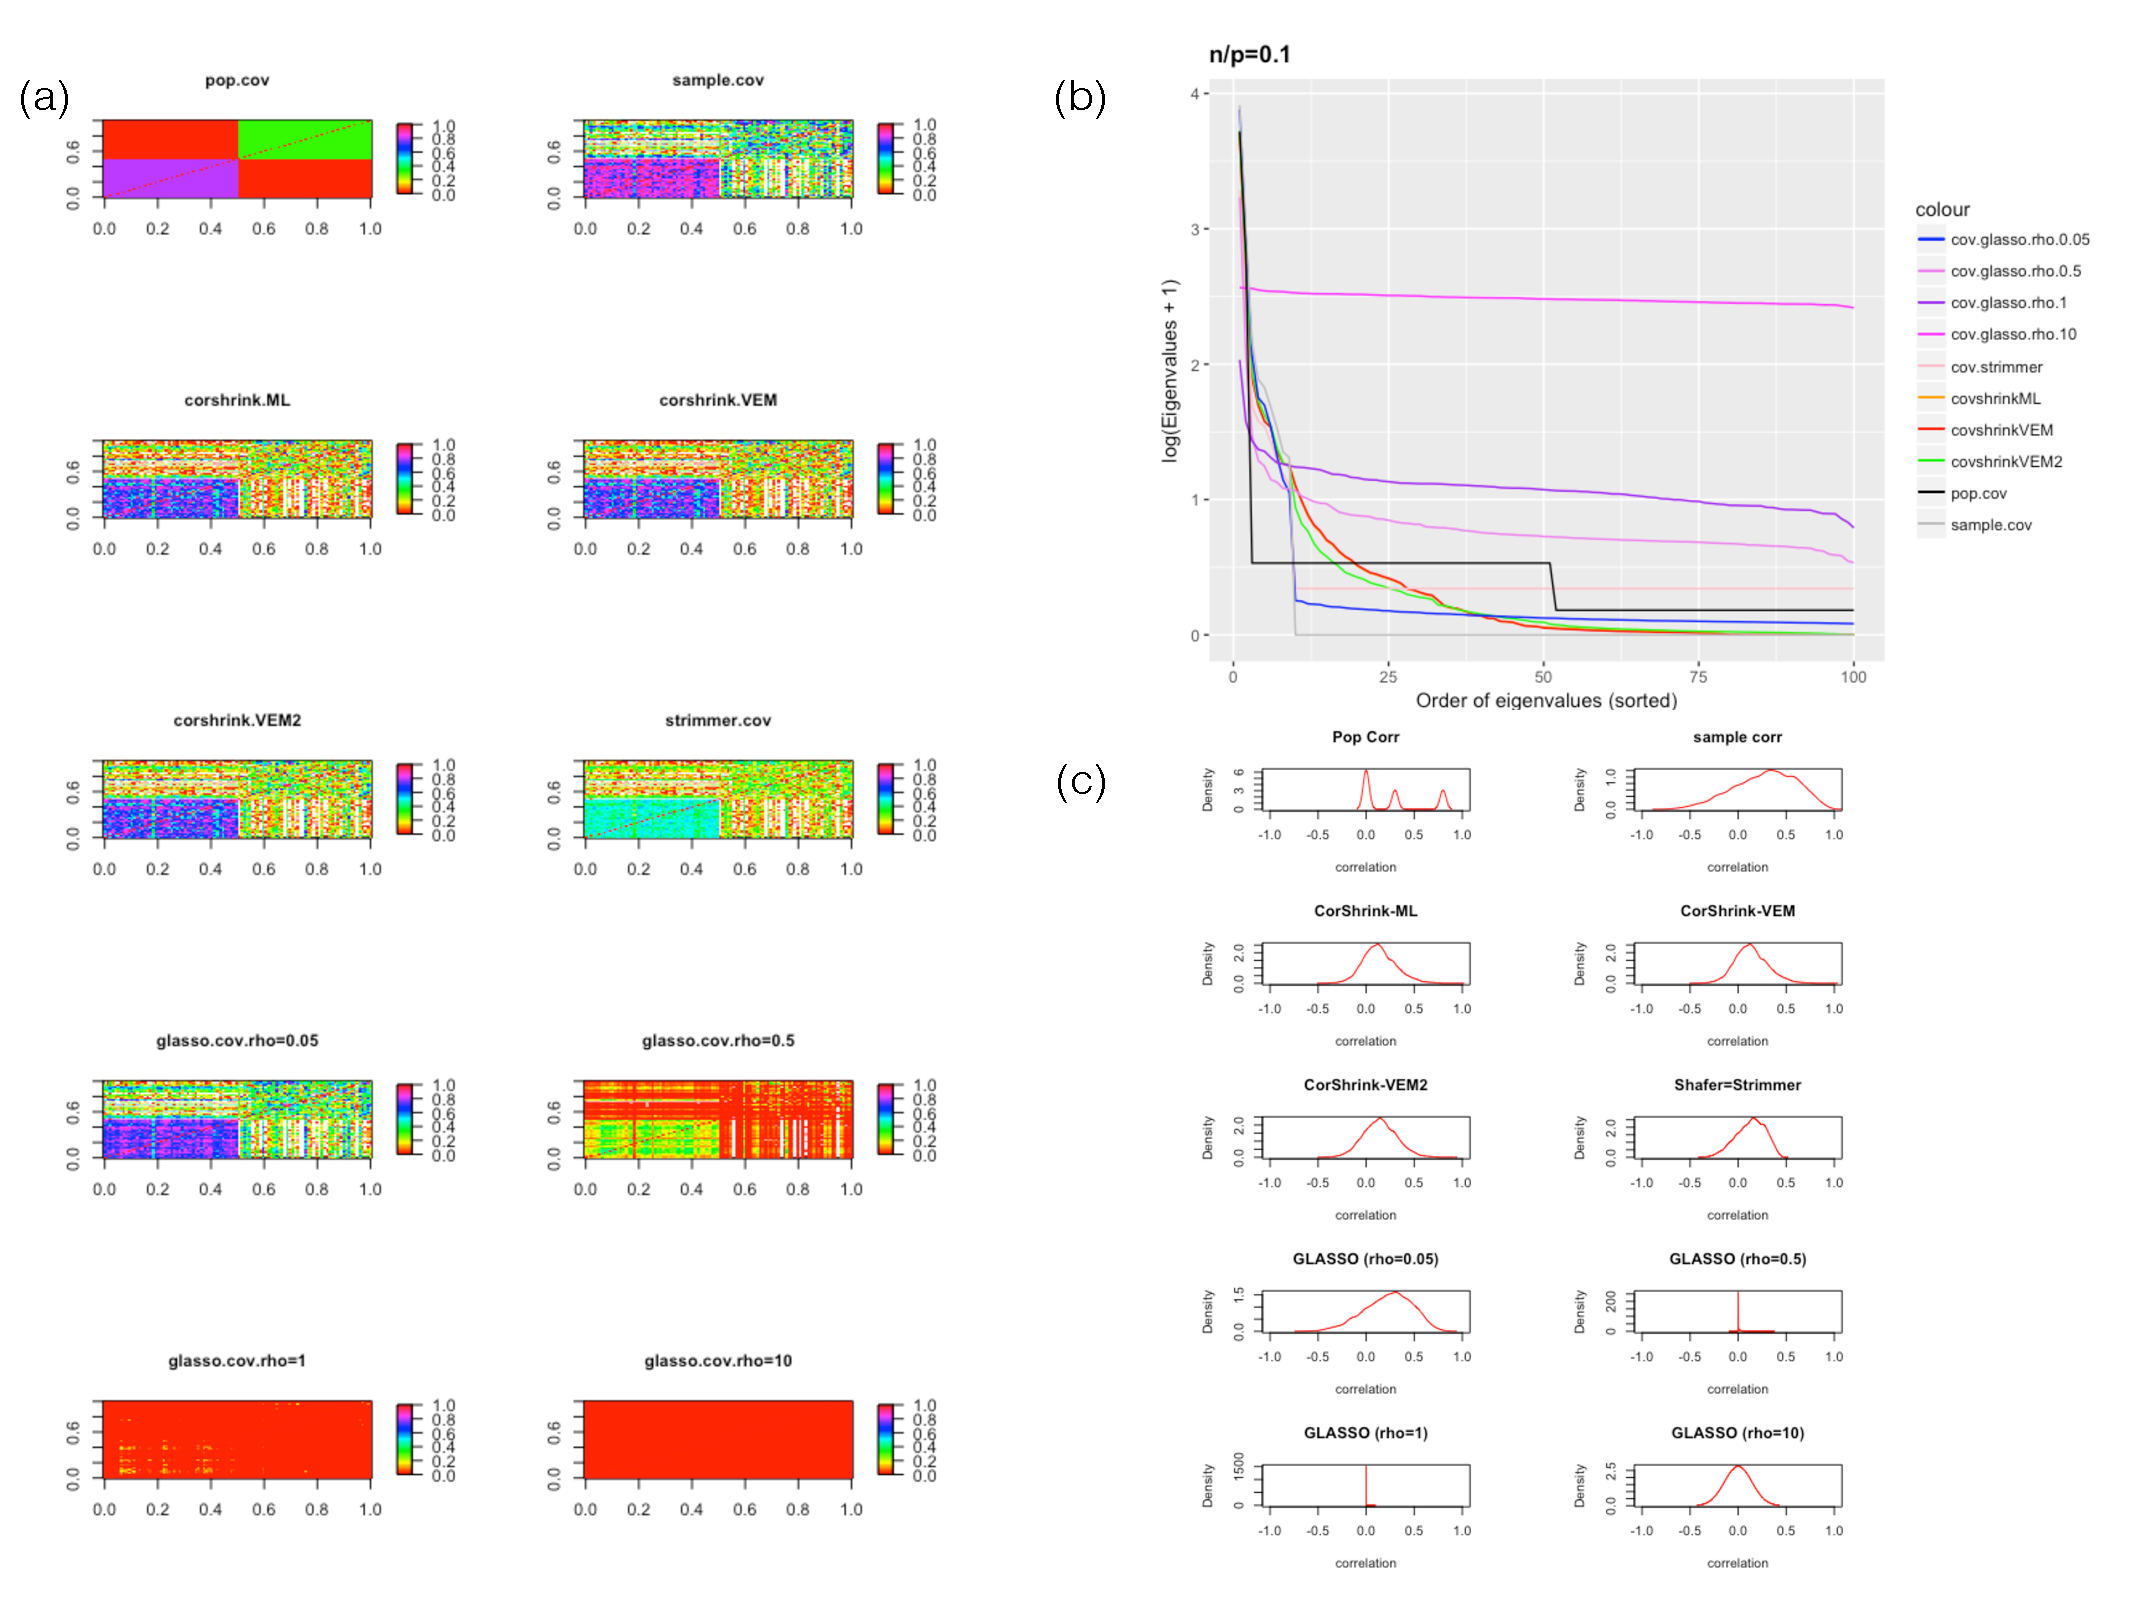
\includegraphics[height=5in, width=7in]{figure1.pdf}
 \caption{\small{Corresponding to 3 versions of \textit{CorShrink}, GLASSO under 4 values of regularization parameters, sample correlation and the population correlation, we show the image plots of the correlation structure in (a). In (b), we display the eigenvalue trends ordered from highest to lowest values for different shrinkage methods and we check how they relate to the original trend for the population correlation matrix. (c) We plot the distributional patterns of the estimated correlations from the different shrinkage methods and compare them with that of the sample correlation and the population correlation}}
\label{fig:fig1}
\end{figure*}

The image plots in Figure \ref{fig:fig1} (a) show that sample correlation fails to approximate the population correlation matrix well in regions of low correlation. The Sch\"{a}fer-Strimmer method, in trying to shrink towards the identity matrix, shrinks the correlations in high correlation regions excessively. The GLASSO method for $0.05$ is very close to the sample covariance matrix, whereas for the other choices, it tends to shrink the correlations too much, demonstrating the sensitivity of GLASSO to the choice of the regularization parameter. Due to the flexibility of the \textit{CorShrink} methods to choose a  target out of a range of possible targets (all of which are noisy versions of identity matrix), it adaptively learns to shrink the correlations. As a result, they enforce more shrinkage on low correlation regions and less shrinkage on the high correlation values compared to the Sch\"{a}fer-Strimmer method and the GLASSO methods. In terms of eigenvalue comparisons in Figure \ref{fig:fig1} (b), \textit{CorShrink} and Sch\"{a}fer-Strimmer shrinkage methods act similarly at the top eigenvalues, but at the lower eigenvalues, the eigenvalue trends become flat for the Sch\"{a}fer-Strimmer shrinkage, while that of a \textit{CorShrink} model forms more of an asymptote. Figure \ref{fig:fig1} (c) shows the distributional profile of the correlation estimates from the different  shrinkage methods. Expectedly the distributions for the shrinkage methods are more concentrated around $0$ compared to sample correlation matrix. While all the methods fail to detect the three peaks of the original matrix, \textit{CorShrink} and Sch\"{a}fer-Strimmer methods show a small bump in the distribution in the region of second mode of the original matrix. The peak extraction power is much better when $n$ is not too small compared to $p$. To see this, the reader can check the correlation distribution plot for $n=50$ and $p=100$ [??here]. 

In the above simulation study, we had a specific block structure to the covariance matrix which resulted in sharp falls initially and flat regions subsequently in the eigenvalue trends. To make a more general comparison, we randomly generated a covariance matrix (using \textbf{clusterGeneration} package by Qiu and Joe (2015) \cite{Qiu2015}) and estimated the corresponding population correlation matrix via different methods . The results are illustrated in Fig \ref{fig:fig2} for $n << p$ scenarios. The \textit{CorShrink} eigenvalue trends seem to follow the population eigenvalue trends closely. Noticeably the top eigenvalues from our approach and the Sch\"{a}fer-Strimmer approach are much closer to the top eigenvalues of the original matrix when compared to estimates from the GLASSO  or the sample correlation matrix. For GLASSO, it seems that increasing the regularization for low $n$ does not affect the top eigenvalues as much as it affects the lower order eigenvalues. This is important since it is usually the top eigenvalues that are of primary interest to researchers in analyzing the structure of dependence.

%
%the eigenvalues of the shrunk covariance matrices under different shrinkage schemes and different choices of $n$ for $p=100$. Results corresponding to other choices of $p$ can be checked here [?Link].    Figure \ref{fig:fig1} shows that the trends of the eigenvalues from the \textit{CorShrink-ML},  \textit{CorShrink-VEM2} and Sch\"{a}fer-Strimmer shrinkage methods are consistently close to the population eigenvalues across all four choices of $n$. The \textit{CorShrink-VEM} version performs well for the $n <<p$ scenarios, however its performance is not so good for moderate to large values of $n$. This is probably due to the fact that for larger data, the strong weight of the Dirichlet hyperprior on the null component and the fixed grid of component variances of underlying mixture model on Fisher Z-scores makes the model inflexible to adapt itself to data, a problem that is solved in VEM2 when the component variances are more flexibly chosen by the model. GLASSO for low shrinkage ( regularization parameter $\rho = 0.05$) is very close to the sample covariance matrix and for high shrinkage ($\rho=10$) provides a matrix close to diagonal and therefore is a bad fit to the population covariance matrix. The $\rho=0.5$ or $\rho = 1$ provide slightly better fit to the population covariance matrix in terms of eigenvalue patterns, but noticeably, for $n << p$ cases, the top eigenvalues (with the highest magnitude) remain very close to that of the sample covariance matrix despite increasing the level of shrinkage and it is the lower order eigenvalues that adapt more rapidly with increasing $\rho$. Here we must emphasize that usually, the top few eigenvalues are of principal interest to researchers interested in lower dimensional representation, and under $n << p$ scenario, the three versions of the \textit{CorShrink} approach and the Sch\"{a}fer-Strimmer shrinkage method are more effective than GLASSO in mapping the top eigenvalues close to the ones from the population covariance matrix. 
%
%The sample covariance matrix  for $n <<p$ has few non-zero eigenvalues since its rank is $\leq n$, and therefore, fits the population eigenvalue structure badly. 

\begin{figure*}[ht]
\raggedleft
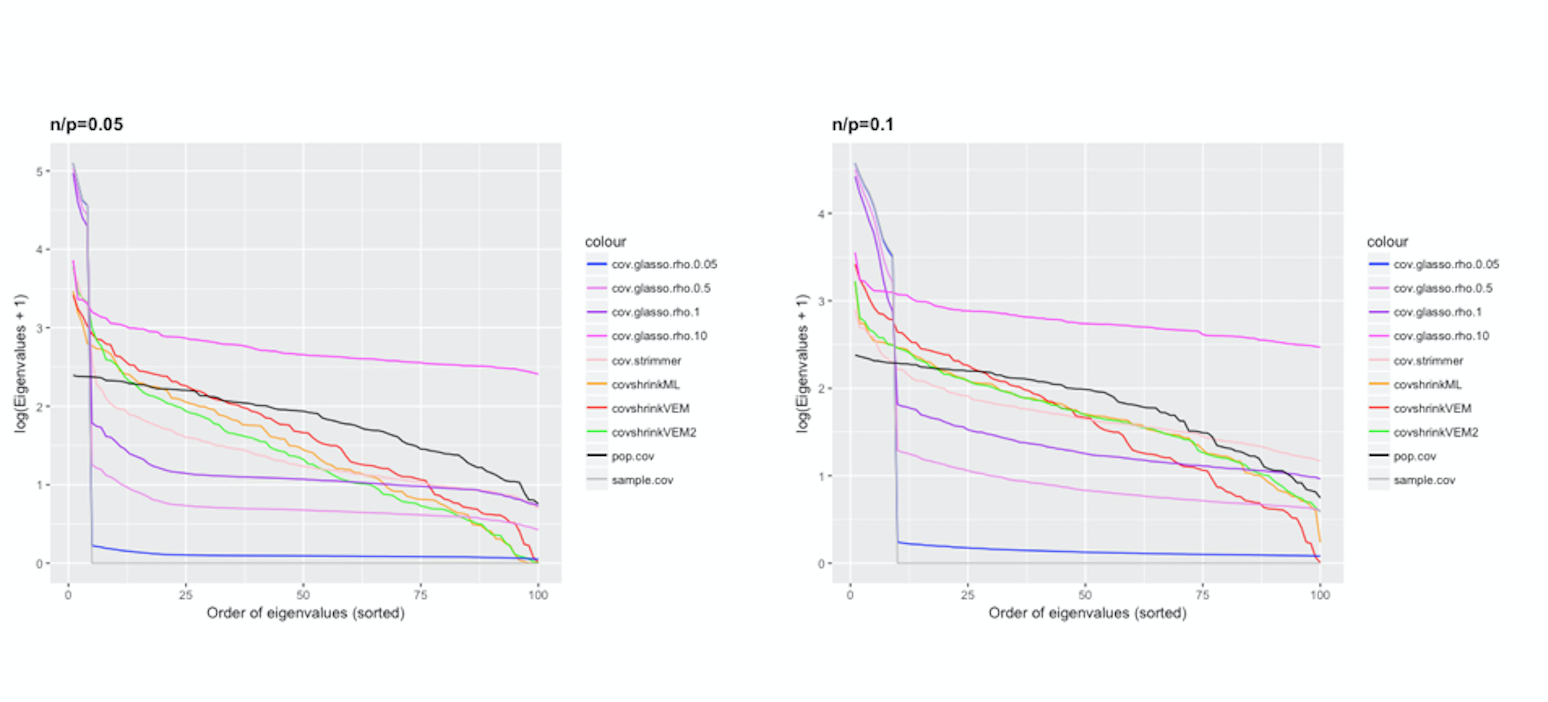
\includegraphics[height=3.5in, width=6in]{figure2a.png}
 \caption{\small{The eigenvalue trends from highest to lowest eigenvalue for $n=5, p=100$ and $n=10, p=100$ for a randomly generated covariance matrix with a smoothly decaying trend in eigenvalues from highest to lowest. }}
\label{fig:fig2}
\end{figure*}

%Besides the eigenvalue trends and the top few eigenvalues, another important consideration in comparing these shrinkage methods is how close the eigenvectors from the shrunk covariance matrices are with respect to the population covariance matrix. Table ~\ref{tab:tab1} present the average distance between the top 5 eigenvectors of the each shrinkage method with respect to the population covariance. Again we find that the Sch\"{a}fer-Strimmer, \textit{CorShrink-ML} and \textit{CorShrink-VEM2}  produce shrunk covariance matrices closest to the population covariance matrix in terms of the eigen-spaces corresponding to the top eigenvalues. In Figure \ref{fig:fig2}, we plot the distribution of the correlations from the shrunk matrices obtained using different shrinkage methods . We observed that the distribution is more concentrated around $0$ for the  \textit{CorShrink} models when compared to the GLASSO and Sch\"{a}fer-Strimmer methods. Additionally,  \textit{CorShrink} retains some correlation values with large magnitudes. This characteristic of the  \textit{CorShrink} approach would ensure a sparse representation when used in building correlation networks.



%
%\begin{figure*}[ht]
%\centering
%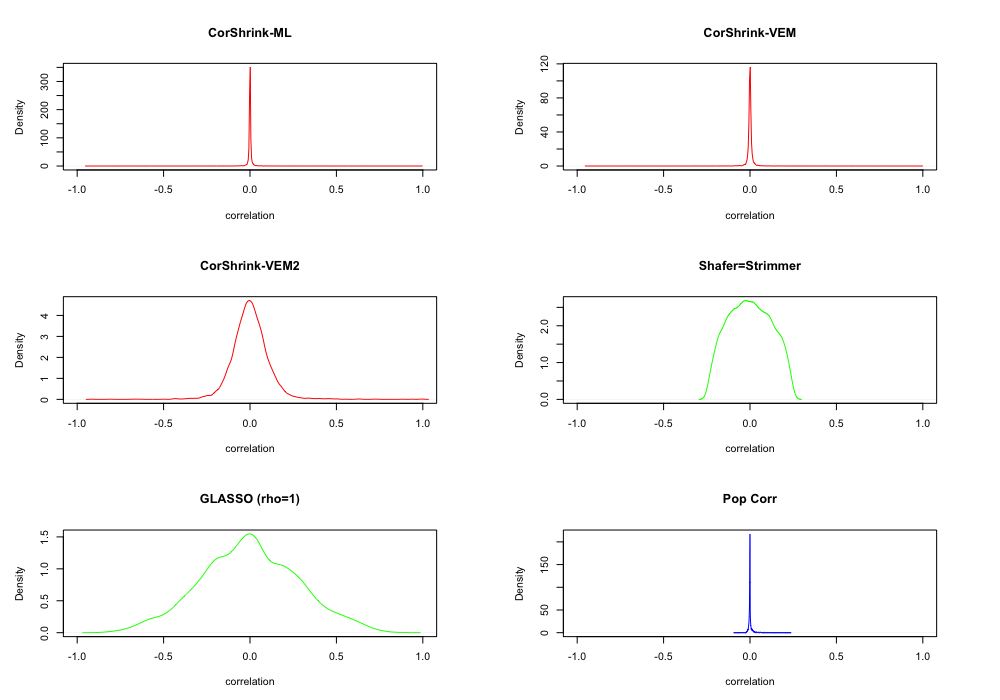
\includegraphics[height=2.5in, width=5in]{correlation_density_compare}
% \caption{Overall distribution of the correlations after shrinking the covariance matrix using the three models of \textit{CorShrink}, Sch\"{a}fer-Strimmer method and the GLASSO method for regularization parameter of $1$ (which was found to be the best fit in terms of eigenvalue patterns out of the four choices considered). The correlation distributions are compared with the actual correlation distribution from the population covariance matrix.}
%\label{fig:fig2}
%\end{figure*}

%\clearpage
%\begin{table}[ht]
%\begin{center}
%\caption{Average Distance of the first 5 eigenvectors of the shrunk covariance matrices from different shrinkage methods versus population covariance matrices. \label{tab:tab2}}
%\begin{tabular}{|p{1.5in}|p{0.8in}|p{0.8in}|p{0.8in}|p{0.8in}|}
% \hline
% Methods &  $n/p=0.05$ & $n/p=0.1$ & $n/p=0.5$ & $n/p=2$ \\ \hline
% CorShrink-ML & 0.030 &  0.034  &  0.033  &  0.036 \\ \hline
% CorShrink-VEM  &  0.037  &  0.039  & 0.057  & 0.062 \\ \hline
% CorShrink-VEM2 & 0.031 & 0.046 & 0.043 & 0.037 \\ \hline
% Sch\"{a}fer-Strimmer & 0.037 & 0.054 & 0.051 &  0.044 \\ \hline
% GLASSO ($\rho=0.05$) & 0.083 & 0.085 & 0.085 & 0.069 \\ \hline
% GLASSO ($\rho=0.1$) & 0.078 & 0.083 & 0.084 & 0.061 \\ \hline
% GLASSO ($\rho=0.5$) & 0.064 & 0.081 & 0.081 & 0.057 \\ \hline
% GLASSO ($\rho=1$) & 0.063 & 0.079 & 0.080 & 0.057 \\ \hline
% Sample cov  & 0.083 & 0.084 & 0.085 & 0.076 \\ 
% \hline	
%\end{tabular}
%\end{center}
% \end{table}
% 

\subsection{Real data application}
Deng et al (2014) \cite{Deng2014} collected single-cell expression data of mouse preimplantation embryos from the zygote to blastocyst stage, with a number cells sequenced at each stage. In total, 259 cells were sequenced and the RNA-seq data was collected over 22431 genes. Transcription factor genes were found to play an important role in clustering the developmental phases from a previous study by Dey et al (2016) \cite{Dey2016}. $1281$ genes from the Deng et al data matched with the Transcription Factor database at \url{http://www.bioguo.org/AnimalTFDB/species.php?spe=Mus_musculus} (see Zhang et al (2012) \cite{Zhang2012}). We applied the \textit{CorShrink-ML} method both ways - on cells and on genes with the aim to determine cell-cell or gene-gene grouping patterns in the data. 

We first apply our methods on the covariance matrix of the $259$ cells. In this case, the genes may be treated as  samples, but they are correlated due to having same transcription factor or being part of the same pathway and this makes it hard to decide on the effective number of independent samples $n$ to use in the model for shrinking correlations. We performed PCA and applied broken stick model to determine first $9$ PCs as signal and used $n=9$ in our model. Figure~\ref{fig:fig3}  shows the image plots of the sample correlation matrix and the \textit{CorShrink-ML} method along with the PC1 vs PC2 plots applied to the estimated matrices respectively. The image plot for the \textit{CorShrink-ML} estimate appears less noisy than the sample correlation image plot and the blocks of (8cell,16 cell) and the blastocysts are more easily discernible in our case. For the PCA plot, the distinction between the cell development phases is still discernible after shrinkage but expectedly, the relative distances between the phases has shrunk. The results for the \textit{CorShrink-VEM} and \textit{CorShrink-VEM2} were very similar to that of \textit{CorShrink-ML} method.

\begin{figure*}[ht]
\raggedleft
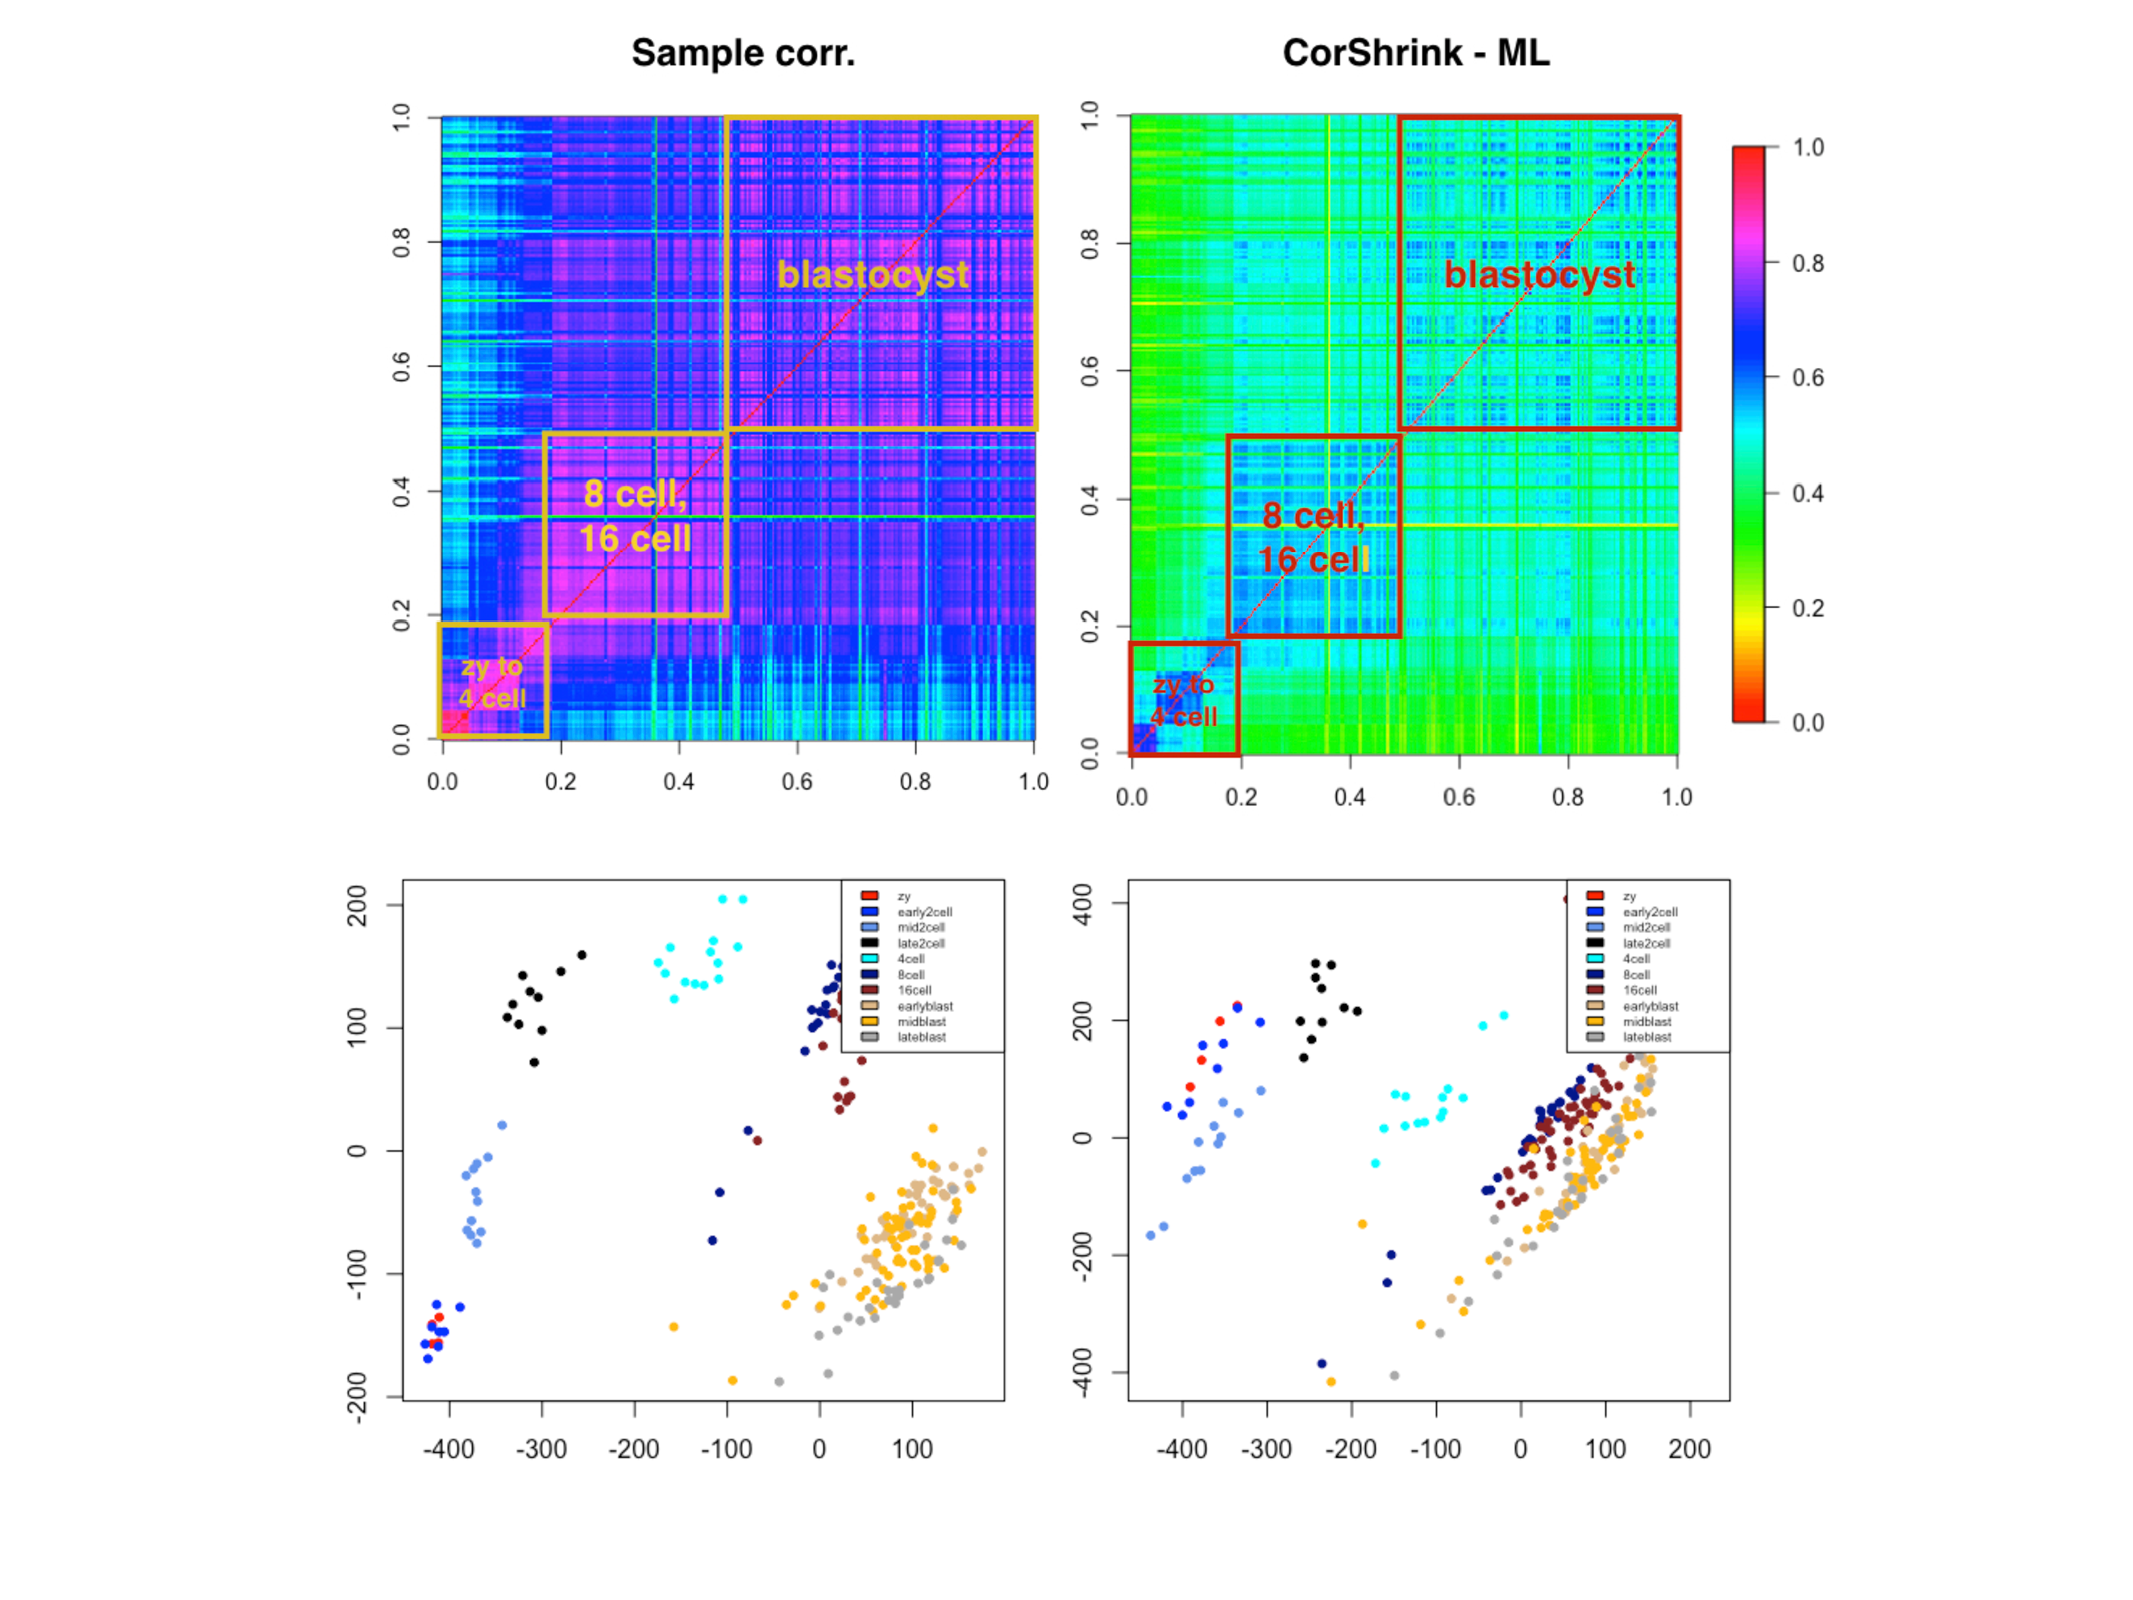
\includegraphics[height=3in, width=6in]{figure3.pdf}
 \caption{\small{The image plot and the PC1 vs PC2 plot of the sample correlation matrix and the estimated correlation matrix obtained using \textit{CorShrink-ML} method.}}
\label{fig:fig3}
\end{figure*}


A more interesting application of our model lies in estimating the gene-gene correlation matrix from the $259$ samples which corresponds to $n << p$ scenario. To do so, we first eliminated genes which have shown non-zero expression in less than $10$ samples. This was aimed at removing expression spiking bias due to sequencing or library preparation biases. After filtering, we were left with $933$ genes on which we applied the \textbf{CorShrink-ML} model. From Figure \ref{fig:fig4}, we find that \textbf{CorShrink-ML} tends to shrink the low to medium correlations significantly while retaining the very strong correlations. We observed the pattern of gene expression across samples for the genes that appear highly correlated among each other in the heatmap (corresponding to upper right corner of the heatmap in Figure \ref{fig:fig4}). We also performed functional annotation enrichment for these genes relative to all other genes that formed the background. The top GO annotations enriched in these genes corresponded to hippocampus,  limbic system and hind brain development (GO:0021766 , GO:0021761,  GO:0030902 ). 

\begin{figure*}[h]
\raggedleft
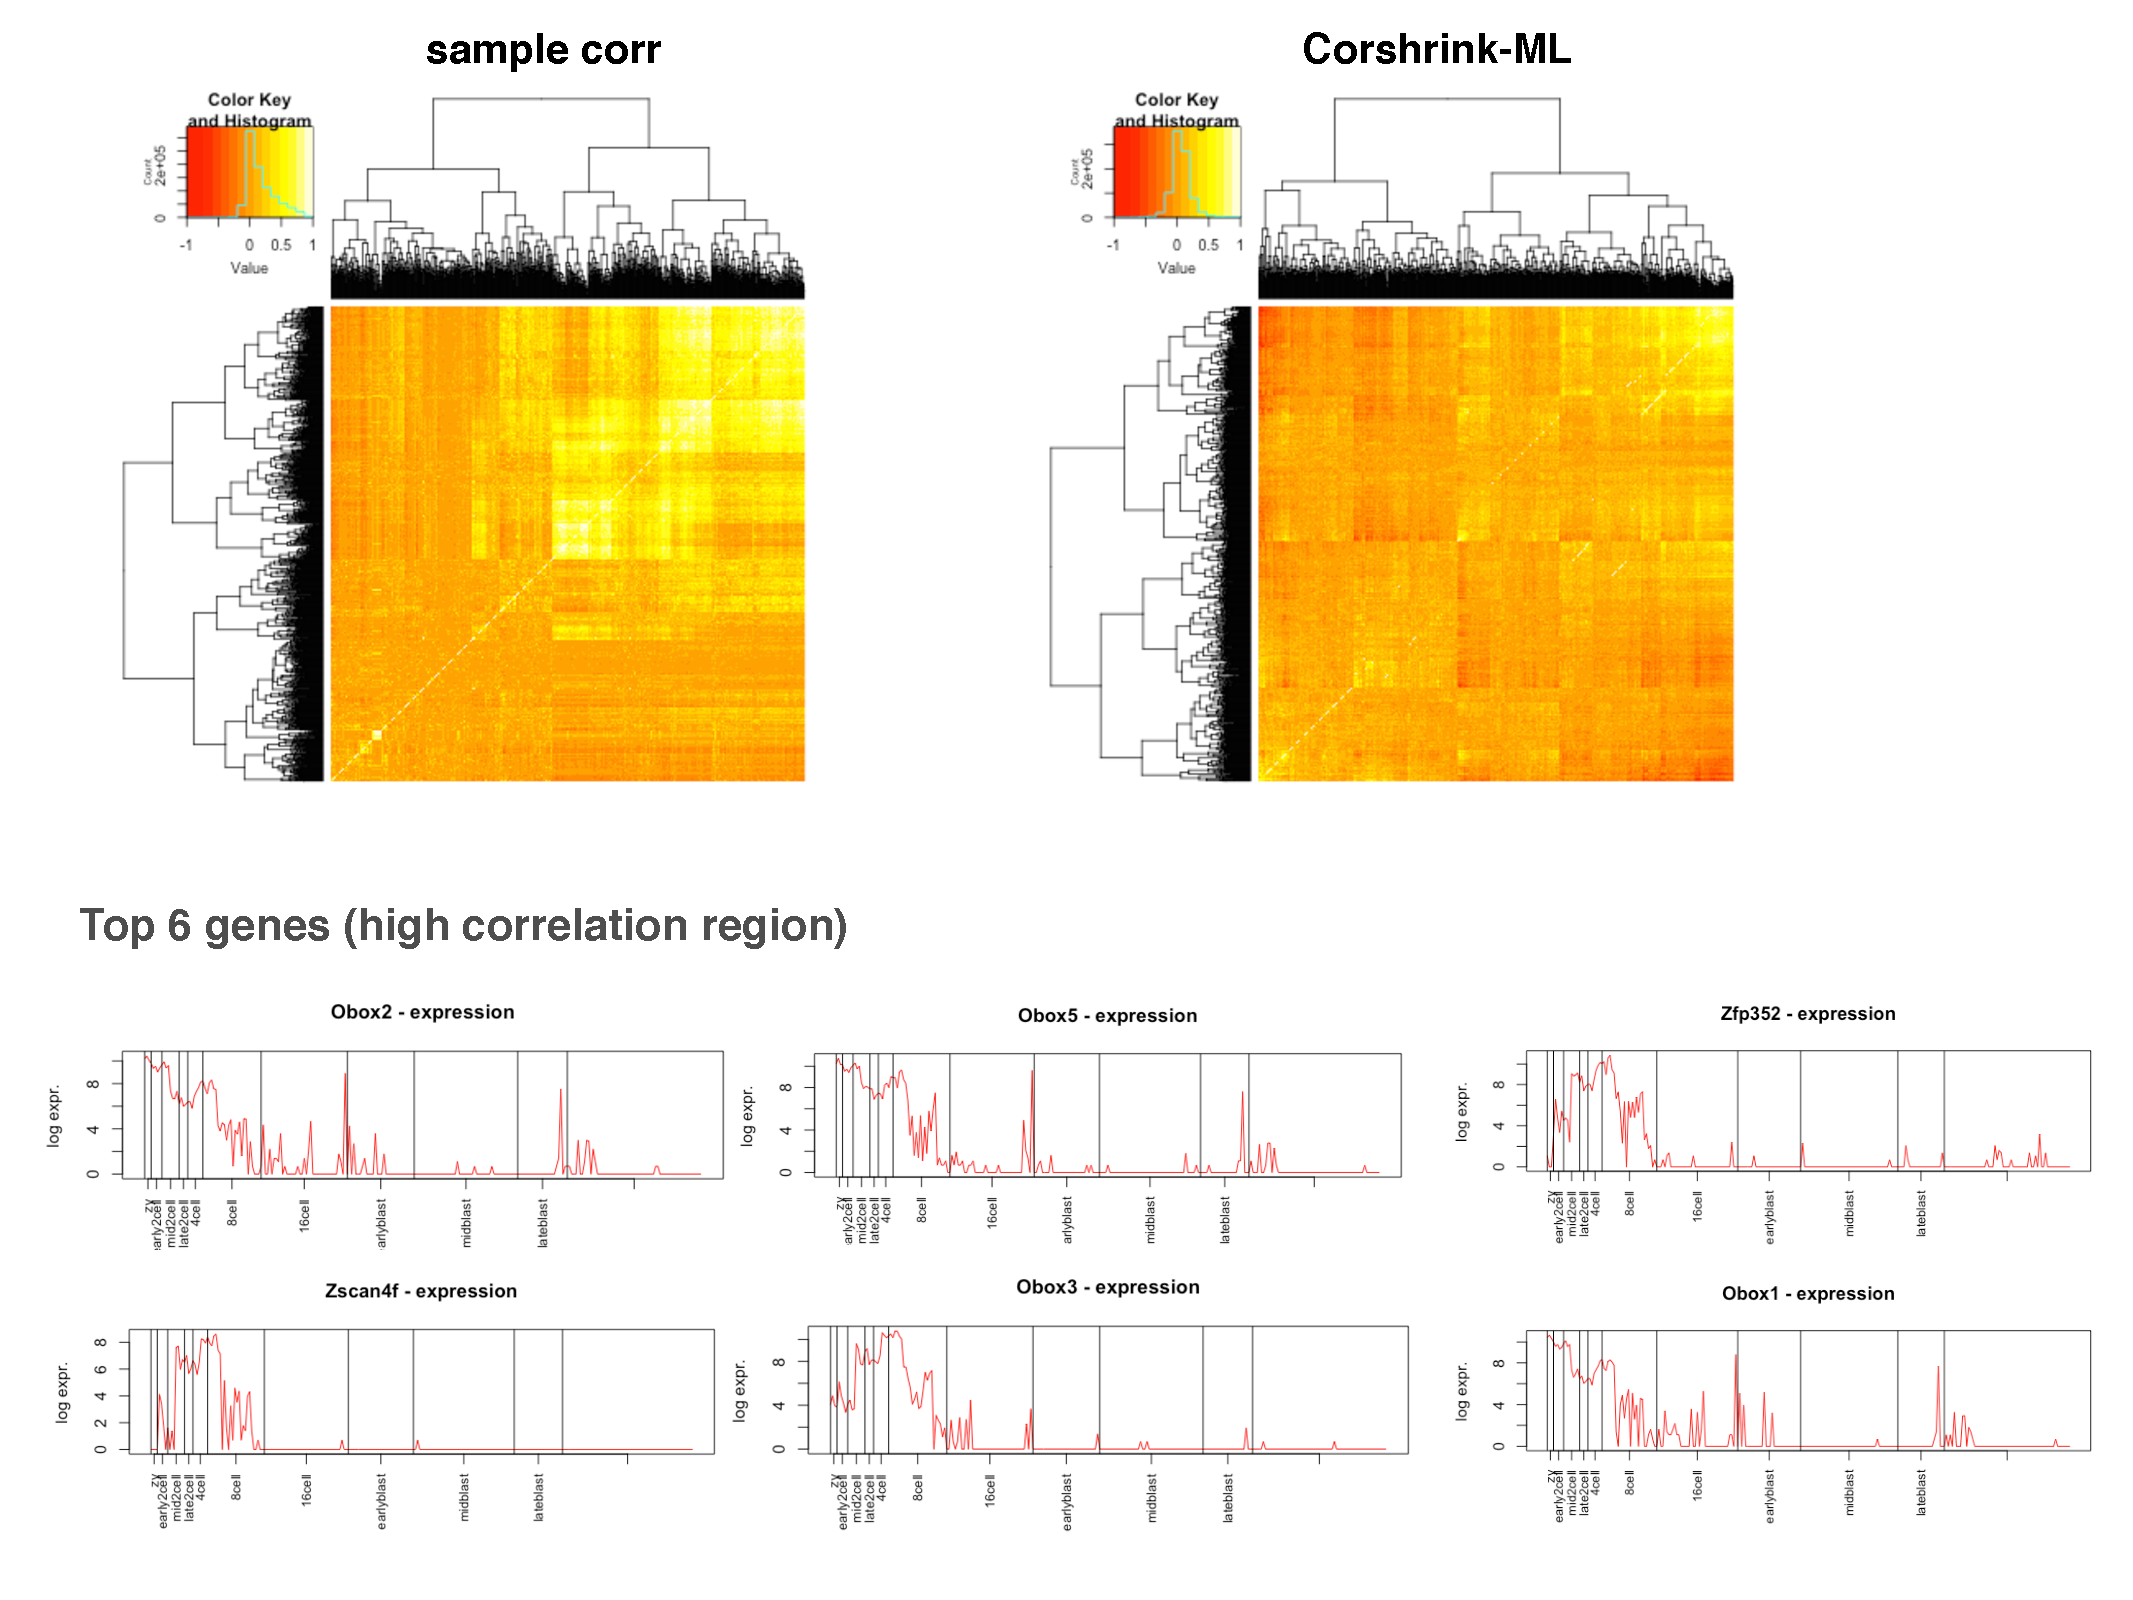
\includegraphics[height=4.5in, width=6in]{figure4.pdf}
 \caption{\small{The heatmap representation of the sample correlation matrix and the \textit{CorShrink-ML} estimated correlation matrix for the TF genes in Deng et al 2014 data \cite{Deng2014}. We investigated the high correlation region at the top right corner of the heatmap and extracted top $6$  most highly correlated genes. All of them showed decreasing trends of log expression from early stages of development (zygote, 2 cell) to the late stages.}}
\label{fig:fig4}
\end{figure*}

\section{Discussion}
 
Our goal here is to highlight the potential of the \textit{CorShrink} models as covariance or correlation shrinkage methods which has more flexibility in choosing the amount of shrinkage for the high and low sample correlations, compared to the 
Sch\"{a}fer Strimmer shrinkage approach (see Figure \ref{fig:fig1}). Also our methods outperform GLASSO as a covariance shrinkage estimator  irrespective of the choice of regularization parameter used for the latter (see Figure~\ref{fig:fig1} and Figure~\ref{fig:fig2}). 

In terms of computational time, the \textit{CorShrink-ML} method is faster than the  \textit{CorShrink-VEM} and \textit{CorShrink-VEM2} methods. For instance, the time taken to run \textit{CorShrink-ML}, \textit{CorShrink-VEM} and \textit{CorShrink-VEM2} on the $259$ samples were  9 seconds,  44 seconds  and 3.1minutes  
respectively.

This method also opens other areas of applications and extensions that we intend to pursue in future. The \textit{CorShrink} models can be easily extended to partial correlation and partial covariance matrices and also facilitate efficient computation of the inverse correlation and covariance matrices. One can create causal networks based on the \textit{CorShrink} models and compare them to the GLASSO based causal networks. Additionally, one can combine Linear Discriminant Analysis and  Multiple regression problem with the estimated covariance matrices obtained from the \textit{CorShrink} models, in the same way the Sch\"{a}fer Strimmer method has been used in these domains \cite{Xu2009} \cite{Schafer2005}. Also for structured covariance matrices, one would want to pool the knowledge of the underlying structure into the shrinkage method. For example, for a block covariance matrix, it makes more sense to apply \textit{CorShrink} separately on each block and pool the blocks together. 

The codes to fit the \textit{CorShrink} models on data are implemented in an R package \textbf{CorShrink} which is available on Github at \url{https://github.com/kkdey/CorShrink}. It also contains a README demonstrating how these models were fitted on simulated data. The Deng et al single cell data \cite{Deng2014} is available as a R data package with instructions for downloading and loading into R at \url{https://github.com/kkdey/singleCellRNASeqMouseDeng2014}.
The scripts to recreate the results and the figures are available in the Github repo \url{https://github.com/kkdey/CorShrink-paper}. 

\begin{thebibliography}{9}

\bibitem{Beal2003}
Beal MJ, Ghahramani Z.
The Variational Bayesian EM Algorithm for Incomplete Data: with Application to Scoring Graphical Model Structures
\textit{Bayesian Statistics}, 7.


\bibitem{Blei2016}
Blei DM, Kucukelbir A, McAuliffe JD. 2016.
Variational Inference: A Review for Statisticians.
https://arxiv.org/pdf/1601.00670.

\bibitem{Deng2014}
Deng Q,  Ramskold D,  Reinius B,  Sandberg R. 2014.
Single-Cell RNA-Seq Reveals Dynamic, Random Monoallelic Gene Expression in Mammalian Cells.
\textit{Science}.  343 (6167) 193-196.

\bibitem{Dey2016}
Dey KK,  Hsiao CJ,  Stephens M. 2016.
Clustering RNA-seq expression data using grade of membership models
\textit{http://biorxiv.org/content/early/2016/05/03/051631}

\bibitem{Friedman2008}
Friedman J,  Hastie T,  Tibshirani R. 2008.
Sparse inverse covariance estimation with the graphical lasso. 
\textit{Biostatistics}. 9.3.

\bibitem{Lancewiki2014}
Lancewicki T. and Aladjem M. 2014.
Multi-Target Shrinkage Estimation for Covariance Matrices.
\textit{IEEE Transactions on Signal Processing}. 62 (24), 6380-6390

\bibitem{Ledoit2003}
Ledoit O. and Wolf  M. 2003. 
"Improved estimation of the covariance matrix of stock returns with an application to portofolio selection.
\textit{Journal of Empirical Finance}. 10 (5): 603?621.

\bibitem{Ledoit2004}
Ledoit O. and Wolf  M. 2004. 
Honey, I shrunk the sample covariance matrix.
\textit{The Journal of Portfolio Management}. 30 (4): 110?119.

\bibitem{Qiu2015}
Qiu W, Joe H. 2015.
clusterGeneration: Random Cluster Generation (with Specified Degree of Separation).
R package version 1.3.4.

\bibitem{Schafer2005}
Sch\"{a}fer J and Strimmer K.  2005. 
A shrinkage approach to large-scale covariance matrix estimation and implications for functional genomics. 
\textit{Statist. Appl. Genet. Mol. Biol}.4.32.

\bibitem{Schafer2005b}
Sch\"{a}fer J and Strimmer K.  2005. 
An empirical Bayes approach to inferring large-scale gene association networks. 
\textit{Bioinformatics}. 21: 754-764.

\bibitem{Stephens2016}
Stephens M. 2016. 
False discovery rates: a new deal. 
\textit{Biostatistics} Advance Access.

\bibitem{Witten2010}
Witten DM,  Friedman JH, Simon N. 2010.
New Insights and Faster Computations for the Graphical Lasso. 
\textit{Journal of Computational and Graphical Statistics}, 20, 4, 892?900.

\bibitem{Xu2009}
Xu P.,  Brock GN,  Parrish RS.  2009.
Modified linear discriminant analysis approaches for classification of high-dimensional microarray data.
\textit{Computational Statistics $\&$ Data Analysis}. 53.5.

\bibitem{Zhang2012}
Zhang HM, Chen H, Liu W, Liu H, Gong J, Wang H and Guo AY. (2012 database issue)
\textit{Nucl. Acids Res}. doi: 10.1093/nar/gkr965

\end{thebibliography}



